\documentclass[12pt]{article}
\newcommand{\HeaderTitle}{Datenbanksysteme 03}
%Begin----------------------------------------------------------------------------------------------------------------------------------------
%---------------------------------------------------------------------------------------------------------------------------------------------


%Package import and Config of Packages
%\usepackage[utf8]{inputenc}%\usepackage{tikz}#
\usepackage{lmodern}
\usepackage{setspace}
\usepackage{lastpage}
\usepackage{pgfplots} % Fuer Plots
\usepackage{pgfplotstable}
\usepackage{pgfkeys} 
\usepackage{filecontents}
\pgfplotsset{compat = newest}
\usepackage{tikz} % Generell gutes Packet
\usepackage{csvsimple} % Zum CSV auslesen
\usepackage{fancyhdr}
\usepackage{tcolorbox}


\usepackage[ngerman]{babel}
\usepackage{datetime}
\newdateformat{myformat}{\THEDAY{ten }\monthname[\THEMONTH], \THEYEAR}

\usepackage{tikz}
\usetikzlibrary{arrows,shapes.gates.logic.US,shapes.gates.logic.IEC,calc}

\usepackage{subfig}
\usepackage{pdfpages}
\usepackage{subfiles}
\usepackage{titlesec}
\usepackage[pdfborder={0 0 0}]{hyperref}
\usepackage{pdfpages}
\usepackage{verbatim}
\usepackage{geometry}
\geometry{left=20mm, right=20mm, bottom=20mm}

\usepackage{svg}
\usepackage{graphicx}
\graphicspath{{../Bilder/}{Bilder/}}
\svgpath{{../svg/}{svg/}}

\usepackage{xcolor}
\usepackage{listings}

\usepackage[normalem]{ulem}

%End------------------------------------------------------------------------------------------------------------------------------------------
%---------------------------------------------------------------------------------------------------------------------------------------------
%Package import and Config of Packages

%Begin----------------------------------------------------------------------------------------------------------------------------------------
%---------------------------------------------------------------------------------------------------------------------------------------------
%List Configuration for Coding
\usepackage{listings} % Generell Code-Boxen
\usepackage{xcolor} % Fuer extra Farben mit color{}

\colorlet{punct}{red!60!black}
\definecolor{background}{HTML}{EEEEEE}
\definecolor{delim}{RGB}{20,105,176}
\colorlet{numb}{magenta!60!black}

\definecolor{mGreen}{rgb}{0,0.6,0}
\definecolor{mGray}{rgb}{0.5,0.5,0.5}
\definecolor{mPurple}{rgb}{0.58,0,0.82}
\definecolor{backgroundColour}{rgb}{255,255,255}
\lstdefinestyle{CStyle}
{
    backgroundcolor=\color{backgroundColour},   
    frame=single,
    belowcaptionskip=1\baselineskip,
    breaklines=true,
    xleftmargin=\parindent,
    language=C,
    showstringspaces=false,
    basicstyle=\footnotesize\ttfamily,
    keywordstyle=\bfseries\color{magenta},
    commentstyle=\color{mGreen},
    identifierstyle=\color{blue},
    stringstyle=\color{orange},
}   

%End------------------------------------------------------------------------------------------------------------------------------------------
%---------------------------------------------------------------------------------------------------------------------------------------------
%List Configuration for Coding


%Begin----------------------------------------------------------------------------------------------------------------------------------------
%---------------------------------------------------------------------------------------------------------------------------------------------
%More Subsections Configuration
\titleclass{\subsubsubsection}{straight}[\subsection]
\newcounter{subsubsubsection}[subsubsection]
\renewcommand\thesubsubsubsection{\thesubsubsection.\arabic{subsubsubsection}}
\renewcommand\theparagraph{\thesubsubsubsection.\arabic{paragraph}} % optional; useful if paragraphs are to be numbered
\titleformat{\subsubsubsection}
  {\normalfont\normalsize\bfseries}{\thesubsubsubsection}{1em}{}
\titlespacing*{\subsubsubsection}
{0pt}{3.25ex plus 1ex minus .2ex}{1.5ex plus .2ex}


\titleclass{\subsubsubsubsection}{straight}[\subsection]
\newcounter{subsubsubsubsection}[subsubsubsection]
\renewcommand\thesubsubsubsubsection{\thesubsubsubsection.\arabic{subsubsubsubsection}}
\titleformat{\subsubsubsubsection}
  {\normalfont\normalsize\bfseries}{\thesubsubsubsubsection}{1em}{}
\titlespacing*{\subsubsubsubsection}
{0pt}{3.25ex plus 1ex minus .2ex}{1.5ex plus .2ex}

\makeatletter
\renewcommand\paragraph{\@startsection{paragraph}{5}{\z@}%
  {3.25ex \@plus1ex \@minus.2ex}%
  {-1em}%
  {\normalfont\normalsize\bfseries}}
\renewcommand\subparagraph{\@startsection{subparagraph}{6}{\parindent}%
  {3.25ex \@plus1ex \@minus .2ex}%
  {-1em}%
  {\normalfont\normalsize\bfseries}}
\def\toclevel@subsubsubsection{4}
\def\toclevel@paragraph{5}
\def\toclevel@paragraph{6}
\def\l@subsubsubsection{\@dottedtocline{4}{7em}{4em}}
\def\l@subsubsubsubsection{\@dottedtocline{5}{8em}{5em}}
\def\l@paragraph{\@dottedtocline{5}{10em}{5em}}
\def\l@subparagraph{\@dottedtocline{6}{14em}{6em}}
\makeatother

\setcounter{secnumdepth}{5}
\setcounter{tocdepth}{5}

%End------------------------------------------------------------------------------------------------------------------------------------------
%---------------------------------------------------------------------------------------------------------------------------------------------
%More Subsections Configuration


\pagestyle{fancy}
\fancyhf{}


%Begin----------------------------------------------------------------------------------------------------------------------------------------
%---------------------------------------------------------------------------------------------------------------------------------------------
%TitelSeite
\title{\HeaderTitle}
\author{Fabio~Plunser}
\date{\today}
\rhead{\hspace{5px}
\includegraphics[scale=0.2]{Bilder/logo.png}}
\lhead{\HeaderTitle}
\rfoot{Page~\thepage ~of~\pageref{LastPage}}
\lfoot{Plunser~Fabio}
\renewcommand{\headrulewidth}{1pt}
\renewcommand{\footrulewidth}{1pt}



\begin{document}
\pagenumbering{gobble}

\begin{titlepage}
  \maketitle
\end{titlepage}

%End------------------------------------------------------------------------------------------------------------------------------------------
%---------------------------------------------------------------------------------------------------------------------------------------------
%TitelSeite

%Begin----------------------------------------------------------------------------------------------------------------------------------------
%---------------------------------------------------------------------------------------------------------------------------------------------
%Inhaltsverzeichnis
\pagebreak
\thispagestyle{empty}
\renewcommand\contentsname{Inhaltsverzeichnis}
\tableofcontents	
\pagenumbering{gobble}

%End------------------------------------------------------------------------------------------------------------------------------------------
%---------------------------------------------------------------------------------------------------------------------------------------------
%Inhaltsverzeichnis

%Begin----------------------------------------------------------------------------------------------------------------------------------------
%---------------------------------------------------------------------------------------------------------------------------------------------
%Abbildungsverzeichnis
\thispagestyle{empty}
\renewcommand\listfigurename{Abbildungsverzeichnis}
\listoffigures
%End------------------------------------------------------------------------------------------------------------------------------------------
%---------------------------------------------------------------------------------------------------------------------------------------------
%Abbildungsverzeichnis
\renewcommand\lstlistlistingname{Code}
\lstlistoflistings

%Begin----------------------------------------------------------------------------------------------------------------------------------------
%---------------------------------------------------------------------------------------------------------------------------------------------
%Codeverzeichnis
% \renewcommand\lstlistlistingname{Codeverzeichnis}
% \lstlistoflistings
\pagebreak
\pagenumbering{arabic}

%End------------------------------------------------------------------------------------------------------------------------------------------
%---------------------------------------------------------------------------------------------------------------------------------------------
%Codeverzeichnis



%Begin----------------------------------------------------------------------------------------------------------------------------------------
%---------------------------------------------------------------------------------------------------------------------------------------------
%Main
\section{Er-Mapping 1}
Address: \underline{address\_id}, street, number, zip\_code, city, state\\
Customer: \underline{customer\_id} creation\_date\\
PrivatePerson: \dashuline{\underline{customer\_id}}, fristname, lastname, birthday \\
Buisness: \dashuline{\underline{customer\_id}}, name, telephone\_number \\
Order: \underline{order\_id}, order\_date, delivery\_date \\ 
Computer: \underline{serial\_no} \\
Software: \underline{name}, \underline{version}, description \\
OS: \underline{name}, \underline{version}, description \\

\begin{minipage}{0.5\textwidth}
        \centering
        \begin{tabular}{|c|c|c|c|c|c|}
            \hline
            \multicolumn{6}{|c|}{Address}\\
            \hline
            \underline{address\_id} & street & number & zip\_code & city & state \\
            \hline
        \end{tabular}
\end{minipage}
\begin{minipage}{0.5\textwidth}
    \centering
        \begin{tabular}{|c|c|}
            \hline
            \multicolumn{2}{|c|}{Customer}\\
            \hline
            \underline{customer\_id} & creation\_date \\
            \hline
        \end{tabular}
\end{minipage}
\vspace{20px}

\begin{minipage}{0.5\textwidth}
    \centering
    \begin{tabular}{|c|c|c|c|}
        \hline
        \multicolumn{4}{|c|}{PrivatePerson}\\
        \hline
        \dashuline{\underline{customer\_id}} & firstname & lastname & birthday \\
        \hline
    \end{tabular}
\end{minipage}
\begin{minipage}{0.5\textwidth}
    \centering
    \begin{tabular}{|c|c|c|}
        \hline
        \multicolumn{3}{|c|}{Buisness}\\
        \hline
        \dashuline{\underline{customer\_id}} & name & telephone\_number \\
        \hline
    \end{tabular}
\end{minipage}

\vspace{20px}

\begin{minipage}{0.5\textwidth}
    \centering
    \begin{tabular}{|c|c|c|}
        \hline
        \multicolumn{3}{|c|}{Order}\\
        \hline
        \underline{order\_id} & order\_date & delivery\_date \\
        \hline
    \end{tabular}
\end{minipage}
\begin{minipage}{0.5\textwidth}
    \centering
    \begin{tabular}{|c|}
        \hline
        \multicolumn{1}{|c|}{Computer}\\
        \hline
        \underline{serial\_no}\\
        \hline
    \end{tabular}
\end{minipage}

\vspace{20px}
\begin{minipage}{0.5\textwidth}
    \centering
    \begin{tabular}{|c|c|c|}
        \hline
        \multicolumn{3}{|c|}{Softare}\\
        \hline
        \underline{name} & \underline{version} & description\\
        \hline
    \end{tabular}
\end{minipage}
\begin{minipage}{0.5\textwidth}
    \centering
    \begin{tabular}{|c|c|c|}
        \hline
        \multicolumn{3}{|c|}{OS}\\
        \hline
        \underline{name} & \underline{version} & description\\
        \hline
    \end{tabular}
\end{minipage}



\newpage
\section{Er-Mapping 2}
User: \underline{user\_id}, username, email, description, data\_registered, noWrittenTexts \\
follows: \dashuline{\underline{user\_id}}, timestamp \\
Test: \underline{text\_id}, timestamp, text \\


\newpage
\section{Er-Daigramm}
    \begin{figure}[!htb]
        \centering
        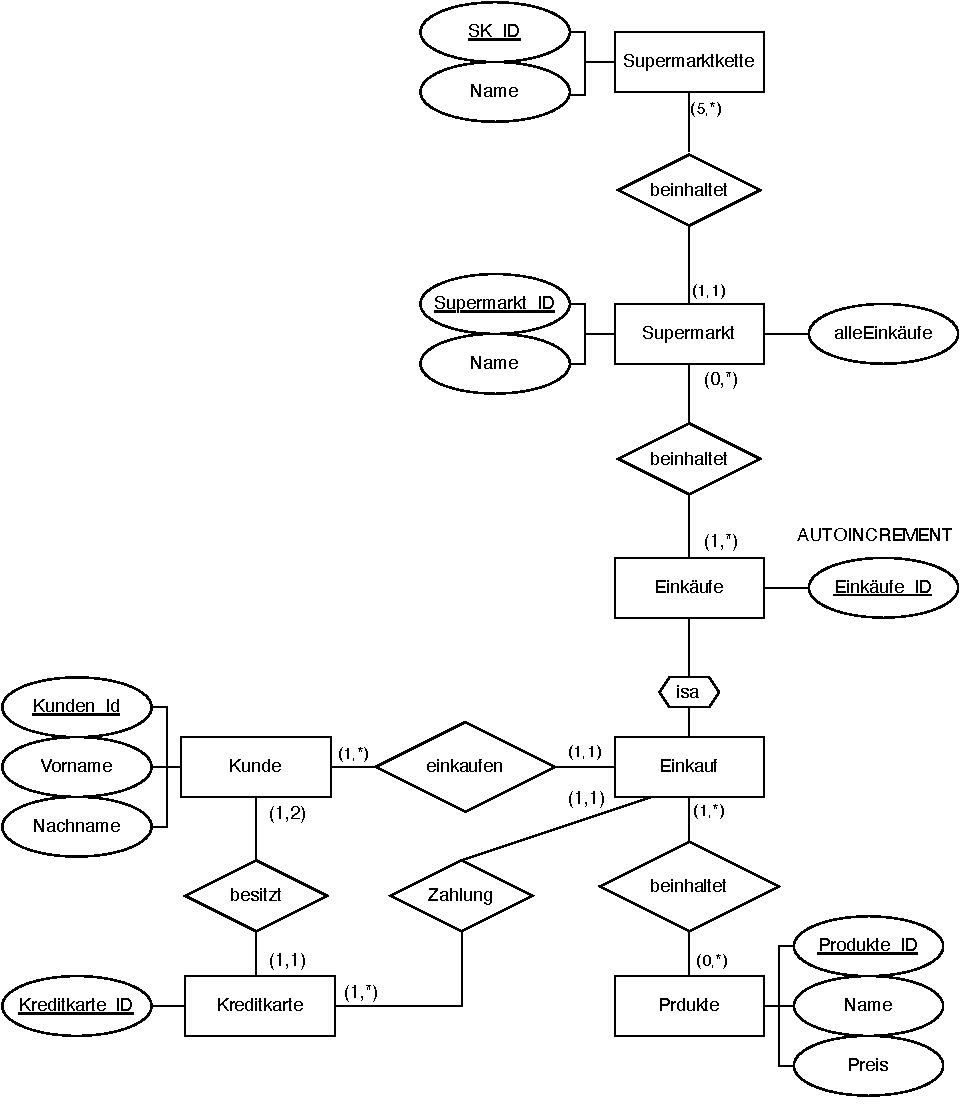
\includegraphics[scale=1]{ER.pdf}
        \caption{ER-Diagramm-Supermarktkette}
        \label{caption:ER-Diagramm-Supermarktkette}
    \end{figure}
    

\newpage{}
\section{ER-Mapping 3}
Kunden: \underline{Kunden\_ID}, Vorname, Nachname \\
Kreditkarte: \underline{Kreditkarder\_ID} \\
Einkauf: \dashuline{\underline{Einkäufe\_ID}}, Uhrzeit \\
Produkte: \underline{Produkt\_ID}, Name, Preis \\
Einkäufe: \underline{Einkäufe\_ID} \\
Supermarkt: \underline{Supermarkt\_ID}, Name, alleEinkäufe \\ 
Supermarktkette: \underline{Supermarktkette\_ID}, Name



%End------------------------------------------------------------------------------------------------------------------------------------------
%---------------------------------------------------------------------------------------------------------------------------------------------
%Codeverzeichnis
\end{document}
